\documentclass{article}
\usepackage{amsmath}
\usepackage{graphicx}
\usepackage[utf8]{inputenc}
\usepackage[bahasai]{babel}
\usepackage{array}

% title
\title{Matematika 1}
\author{Yerri Susatio\\
\emph{Department of Engineering Physics}\\
Institut Teknologi Sepuluh Nopember}
\date{\today}

\numberwithin{equation}{section}
\begin{document}
\maketitle

\section{Persamaan Garis}
\subsection{Bentuk Umum Persamaan Garis}
Bentuk umum persamaan garis lurus adalah sebagai berikut,
\begin{equation}
    ax+by+c = 0
\end{equation}

dimana a, b, c adalah bilangan real.\\
Ubah persamaan diatas menjadi:
$$ by = -ax -c$$ 
Jika kesemua sukunya dibagi dengan $b$ maka,
$$ y = -\frac{a}{b}x - \frac{c}{b}$$
dimana $\cfrac{a}{b}$ merupakan gradien garis = $\arctan \theta=m$\\
$\theta$ = sudut positif antara garis dan sumbu x.\\
\vskip10pt
\begin{tabular}{ l c r }
\raisebox{-.5\height}{\includegraphics[width=2in]{pict/m1}} & & $m = \dfrac{y_B-y_A}{x_B-x_A}=\dfrac{y_A-y_B}{x_A-x_B}$
\end{tabular}

\subsection{Persamaan Garis Lewat ($x_0, y_0$) dengan gradien $m$}
\begin{equation}
    y-y_0=m(x-x_0) \label{pers1_2}
\end{equation}

\subsection{Persamaan garis lewat dua titik($x_a, y_a$), ($x_b, y_b$)}
Gunakan persamaan \ref{pers1_2} untuk memperoleh persamaan garis lewat dua titik sebagai berikut dengan mensubtitusi nilai m menjadi sebagai berikut,
$$y - y_A = \dfrac{y_B - y_A}{x_B - x_A} (x - x_A)$$
\begin{equation}
\dfrac{y-y_B}{y_B - y_A} = \dfrac{x - x_A}{x_B - x_A}
\end{equation}

\subsection{Sudut antara dua garis}
Jika diketahui dua garis, $g$ dan $l$, dimana persamaan keduanya adalah sebagai berikut, \\
$g: \hskip10pt ax + by + c = 0 \rightarrow m_1= - \dfrac{a}{b} $ \\ \\
$l: \hskip10pt px + qy + r = 0 \rightarrow m_2= - \dfrac{p}{q} $ \\ \\
maka sudut antar dua garis tersebut dapat dicari dengan persamaan berikut:\\
$$ \tan \theta = \dfrac{m_1 - m_2}{1+m_1m_2} ~~\Longrightarrow~~Buktikan!!$$

\subsection{Jarak titik($x_0, y_0$) ke garis $ax+by+c=0$} 
Jika $d$ adalah jarak dari titik ($x_0, y_0$) ke garis  $ax+by+c=0$, maka $d$ dirumuskan, \\
\begin{equation}
    d = \Biggl|\dfrac{a.x_0+b.y_0+c}{\sqrt{a^2+b^2}} \Biggr|
\end{equation}

\subsection{Persamaan garis bagi sudut}
Jika diketahui dua gari, $g$ dan $l$, seperti sebelumnya,\\
$g: \hskip10pt ax + by + c = 0 $ \\ 
$l: \hskip10pt px + qy + r = 0 $\\ \\
maka persamaan garis bagi sudut dinyatakan dengan \\
$$\dfrac{ax+by+c}{\sqrt{a^2+b^2}} = \dfrac{px+qy+r}{\sqrt{p^2+q^2}} $$


\subsection{Persamaan berkas garis}
Kembali kita menggunakan dua persamaan gari sebagai berikut, \\
$g: \hskip10pt ax + by + c = 0 $ \\ 
$l: \hskip10pt px + qy + r = 0 $\\ 
Setiap garis yang melewati titik potong kedua garis tersebut, disebut sebagai persamaan berkas garis,
\begin{center}
    \fbox{$g+\lambda{l} = 0$}
\end{center}
dimana $\lambda$ = konstanta yang ditentukan dari syarat sebelumnya.

\subsection{Pergeseran grafik}
\underline{Pergeseran ke kanan - kiri}\\
Perhatikan persamaan garis lurus di bawah ini,\\
\begin{figure}[!h]
    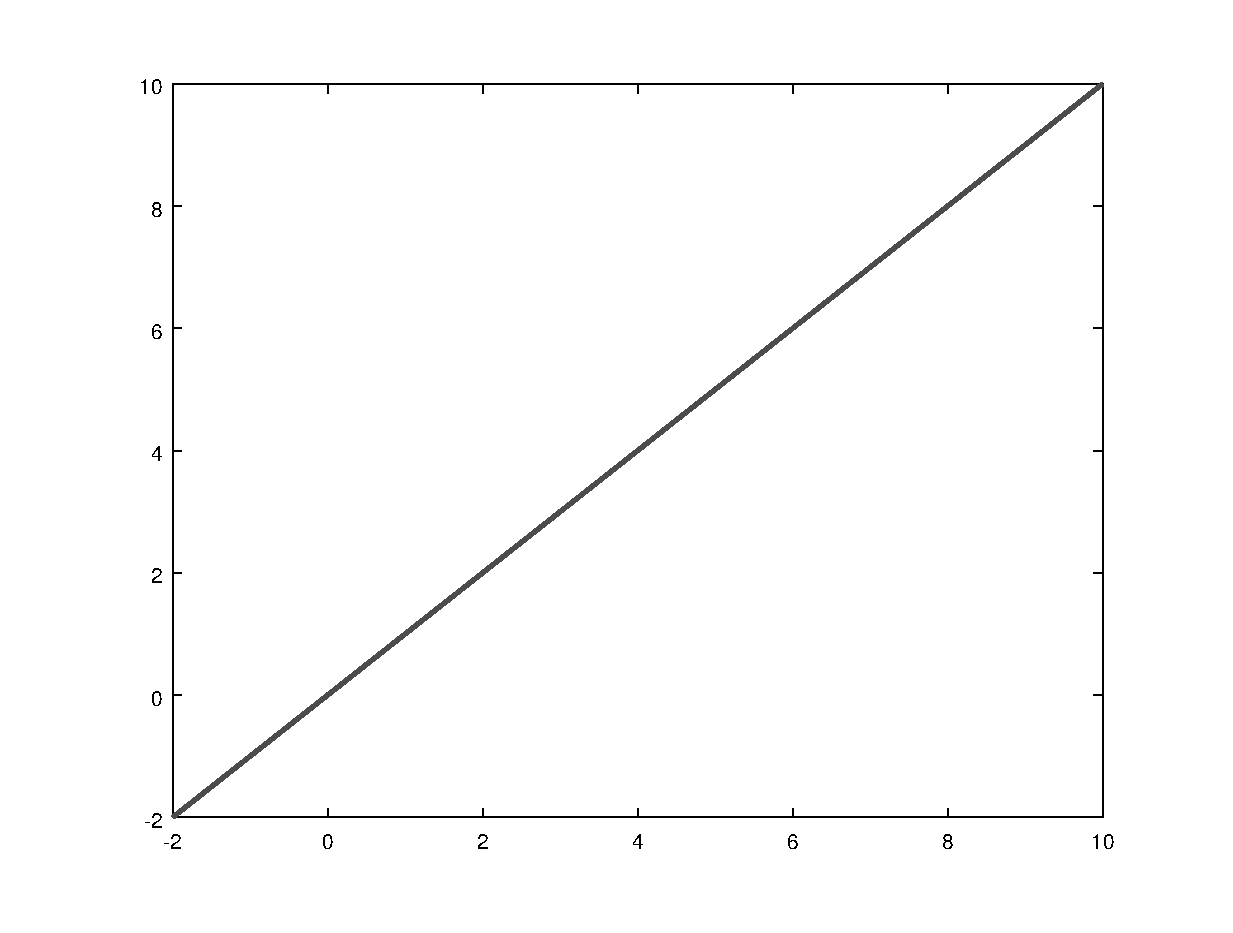
\includegraphics[width=3in]{pict/grafik1}
    \caption{Grafik persamaan garis $y=x$} \label{grafik1}
\end{figure}
Jika setiap titik pada garis tersebut digeser $//$ sumbu x kekanan sejauh 2, maka akan didapatkan pergeseran grafik seperti pada gambar \ref{grafik1-2}\\
\begin{figure}
    \includegraphics[width=4in]{pict/grafik1-2}
        \caption{Grafik persamaan garis $y=x-2$} \label{grafik1-2}
\end{figure}
 \\
asal: $y = x$ \\
Hasil geser:    $y= x-2 $\\
$x \rightarrow (x-2)$\\
$y - 0 = 1(x -2)$\\
$y = x - 2$\\

Jadi pergeseran kekanan sejauh 2, terjadi jika
\begin{center}
    $x \rightarrow (x-2)$
\end{center}


\underline{Soal:}

Garis $y=x+5$ terbentuk jika $y=x$ digeser ke .... sejauh .....\\
 \\
\underline{Pergeseran ke atas - bawah}\\
$y=x$ digeser menjadi $y=x-2$ atau $y+2=x$\\
yang berubah $y \rightarrow (y+2)$\\


\begin{figure}
    \includegraphics[width=4in]{pict/grafik1-3}
        \caption{Grafik persamaan garis $y+2=x$} \label{grafik1-3}
\end{figure}


\subsection{Grafik dengan harga mutlak}

\section{Grafik Parabola}
\subsection{Parabola dengan sumbu simetri sejajar sumbu $x$}

\subsection{Parabola dengan sumbu simetri sejajar sumbu $y$}

\subsection{Bentuk lain persamaan parabola}

\end{document}
